% !TeX spellcheck = en_US

\chapter{Building solution DFAs} \label{ch:2}

\gregor{argue that and why we make A sol complete}

We want an algorithm for DFA generation that fulfills the following conditions:
\begin{itemize}
	\item[->] minimal
	\item[->] number of states
	\item[->] number of \MinMark\ iterations ($\mmD(A_{sol})$)
	\item[->] alphabet size
	\item[->] number of accepting states
	\item[->] planarity (can be checked in $O(|Q_{sol}|)$)
	\item[->] $A_{sol}$ is unused (regarding all previously generated solution DFAs)
\end{itemize}

\begin{definition}[BuildNewMinimalDFA] $ $
	\begin{description}
		
		\item[Given:] $ $
		
		$q, a, f, m_{min}, m_{max} \in \mathbb{N},$
		
		$p \in \{0,1\}$
		\item[Request:] $ $
		
		Let $A_{sol} = (Q, \Sigma, \delta, s, F)$ be a DFA, such that
		
		\qquad $|Q|=q$, $|\Sigma|=a$, $|F|=f$,
		
		\qquad $m_{min} \le \mmD(A_{sol}) \le m_{max}$,
		
		\qquad $A_{sol}$ is planar iff $p = 1$ and
		
		\qquad the language of $L(A)$ is unequal to any DFA used before.
		
		Return $A_{sol}$, if it exists, $\bot$ otherwise.
	\end{description}
\end{definition}

\section{Using trial and error}

We will develop an algorithm that makes partly use of the trial-and-error paradigm to find matching DFAs. The approach here is as follows:

Firstly a \emph{test} DFA $A_{test}$ is generated by use of either randomness or enumeration. Alphabet size and number of (final) states will already be correct. On this DFA then tests will be executed, to check if it is minimal, planar (if wished) and unused. If this is the case, $A_{test}$ will be returned, if not, new test DFAs are generated until all tests pass.

By constructing test DFAs with already correct alphabet size and number of (final) states we are able to subdivide the search space of DFAs in advance into much smaller pieces.

\gregor{How much smaller?}

\vspace{0.2cm}
\begin{algorithmic}[1]
	\Function{BuildNewMinimalDFA-1\ }{$q, a, f, m_{min}, m_{max} \in \mathbb{N}, p \in \{0,1\}$}
		\While {True}
		
			\vspace{0.2cm}
		
			\State generate DFA $A_{test}$ with $|Q|, |\Sigma|, |F|$ matching $q, a, f$
			
			\vspace{0.2cm}
			
			\If {$A_{test}$ not minimal \textbf{or not} $m_{min} \leq \mmD(A_{test}) \leq m_{max}$}
				\State \textbf{continue}
			\EndIf
			
			\If {$p = 1$ \textbf{and} $A_{test}$ is not planar}
				\State \textbf{continue}
			\EndIf
			
			\If {$A_{test}$ was used before}
				\State \textbf{continue}
			\EndIf
			
			\vspace{0.2cm}
			
			\State\Return $A_{test}$
		\EndWhile
	\EndFunction
\end{algorithmic}
\vspace{0.2cm}
We will complete this algorithm by resolving how the tests in lines $4, 6$ and $8$ work and by showing two methods for generation of automatons with given restrictions of $|Q|, |\Sigma|$ and $|F|$.

\subsection{Ensuring $A_{test}$ is minimal and $\mmD(A_{test})$ is correct}

In order to test, whether $A_{test}$ is minimal, we could simply use the minimization algorithm and compare the resulting DFA and $A_{test}$ using an isomorphy test. However it is sufficient to ensure, that no duplicate or unreachable states exist.

To get $\mmD(A_{test})$, we have to run \MinMark\ entirely anyway. Hence we can combine the test for duplicate states with computing the DFAs $\mmD$-value:
\vspace{0.2cm}
\begin{algorithmic}[1]
	\Function{HasDuplicateStates}{$A$}
		\State $depth \gets 0$
		\State $M \gets \{ (p,q), (q,p)\ |\ p \in F, q \notin F \}$
		\Do
			\State $depth \gets depth + 1$
			\State $M' \gets \{ (p,q)\ |\ (p,q) \notin M \land \exists \sigma \in \Sigma \colon (\delta(p,\sigma), \delta(q,\sigma)) \in M \}$
			\State $M \gets M \cup M'$
		\doWhile {$M' \neq \emptyset$}
		\State $hasDupl \gets | \{ (p,q)\ |\ p \neq q \land (p,q) \notin M \} | > 0$
		\State \Return $hasDupl, depth$
	\EndFunction
\end{algorithmic}
\vspace{0.2cm}
Since \MinMark\ computes all non-duplicate state pairs $\neg d_A$, we test in line $9$, whether there is a pair of distinct states not in $\neg d_A$.

Regarding the unreachable states, we can just use \textsc{ComputeUnreachableStates} and test whether the computed set is empty:
\vspace{0.2cm}
\begin{algorithmic}[1]
	\Function{HasUnreachableStates}{$A$}
	\State \Return $|\textsc{ComputeUnreachableStates}(A)| > 0$
	\EndFunction
\end{algorithmic}
\gregor{Is there a more efficient method? Since we actually need to know of only one unreachable state.}

\subsection{Ensuring $A_{test}$ is planar}

There exist several algorithms for planarity testing of graphs. In this work, the library \emph{pygraph}\footnote{\url{https://github.com/jciskey/pygraph}} has been used, which implements the Hopcroft-Tarjan planarity algorithm. More information on this can be found for example in this~\cite{kocay93} introduction from William Kocay. The original paper describing the algorithm is~\cite{hopcroft74}.

\subsection{Ensuring $A_{test}$ is unused}

In our requirements we stated, that we wanted the generated solution DFA to be unused with regards to all previous generated solution DFAs. This implies the need of a database, that allows saving single DFAs and loading DFAs. We name this database \emph{DB1}. Assuming the database is relational, the following scheme is proposed:
\begin{center}
	\begin{tabular}{c c c c c c}
	$|Q_A|$ & |$\Sigma_A$| & $|F_A|$ & $\mmD(A)$ & $isPlanar(A)$ & $encode(A)$
	\end{tabular}
\end{center}
With this scheme we can fetch once all DFAs matching the search parameters. Thus we need not fetch all used DFAs every time, but only those that are relevant. Afterwards we must only check whether any isomorphy test on the current test DFA and one of the fetched DFAs is positive. If any test DFA passes all tests and is going to be returned, then we have to save that DFA in the database.

A more concrete specification of this proceeding is shown below, embedded in the main algorithm:
\vspace{0.2cm}
\begin{algorithmic}[1]
	\Function{BuildNewMinimalDFA-2\ }{$q, a, f, m_{min}, m_{max}, p$}
	
		\vspace{0.2cm}
	
		\State $l \gets$ all DFAs in DB1 matching $q, a, f, m_{min}, m_{max}, p$
		
		\vspace{0.2cm}
		
		\While {True}
		
		\vspace{0.2cm}
		
			\State $\ldots$
			\If {$A_{test}$ is isomorph to any DFA in $l$}
				\State \textbf{continue}
			\EndIf
			
			\vspace{0.2cm}
			
			\State save $A_{test}$ and its respective properties in DB1
			\State\Return $A_{test}$
		\EndWhile
	\EndFunction
\end{algorithmic}
\vspace{0.2cm}

\subsection{Option 1: Generating $A_{test}$ via Randomness}

We now approach the task of generating a random DFA whereas alphabet and number of (final) states are set.

Corollary~\ref{ch:1:cor:all-min-dfa-ism} tells us, that the states names are irrelevant for the minimality of a DFA, therefore we will give our generated DFAs simply the states $q_0, \ldots, q_{q-1}$. For alphabet symbols this is not given. But since we \gregor{TODO minimality and planarity complete under isomorphy}

We can state, that our start state is $q_0 \in Q$, since we apply an isomorphism to every that, such that its start state is relabeled to $q_0$.

The remaining elements that need to be defined are $\delta$ and $F$. The set of final states is supposed to have a size of $f$ and be a subset of $Q$. Therefore we can simply choose randomly $f$ distinct states from $Q$.

The transition function has to make the DFA complete, so we have to choose an ``end'' state for every combination in $Q \times \Sigma$. There is no restriction as to what this end state shall be, so given $q \in Q$ and $\sigma \in \Sigma$ we can randomly choose an end state from $Q$.

With defining how to compute $\delta$ we have covered all elements of a DFA.

\vspace{0.2cm}
\begin{algorithmic}[1]
	\Function{BuildNewMinimalDFA-3a\ }{$q, a, f, m_{min}, m_{max}, p$}
	
		\vspace{0.2cm}
	
		\State $l \gets$ all DFAs in DB1 matching $q, a, f, m_{min}, m_{max}, p$
		\State $Q \gets \{q_0, \ldots, q_{q-1}\}$
		\State $\Sigma \gets \{\sigma_0, \ldots, \sigma_{a-1}\}$
		
		\vspace{0.2cm}
		
		\While {True}
		
		\vspace{0.2cm}
		
			\State $\delta \gets \emptyset$
			\For {$q$ \textbf{in} $Q$}
				\For {$\sigma$ \textbf{in} $\Sigma$}
					\State $q' \gets$ random chosen state from $Q$
					\State $\delta \gets \delta \cup \{((q,\sigma),q')\}$
				\EndFor
			\EndFor
			\State $s \gets 0$
			\State $F \gets$ random sample of $f$ states from $Q$
			\State $A_{test} \gets (Q, \Sigma, \delta, s, F)$
			
			\vspace{0.2cm}
			
			\If {$A_{test}$ not minimal \textbf{or not} $m_{min} \leq \mmD(A_{test}) \leq m_{max}$}
			\State \textbf{continue}
			\EndIf
			
			\If {$p = 1$ \textbf{and} $A_{test}$ is not planar}
			\State \textbf{continue}
			\EndIf
			
			\If {$A_{test}$ is isomorph to any DFA in $l$}
			\State \textbf{continue}
			\EndIf
			
			\vspace{0.2cm}
			
			\State save $A_{test}$ and its respective properties in DB1
			\State\Return $A_{test}$
		\EndWhile
	\EndFunction
\end{algorithmic}
\vspace{0.2cm}

\subsection{Option 2: Generating $A_{test}$ via Enumeration}

% enumerating instead of random

The second method of test DFA generation is based on the idea, that instead of randomly generating $F$ and $\delta$, we could just enumerate through all possible final state sets and transition functions.

% finite enumerations, how many

Both enumerations are finite, given $q$ and $a$. Having a requirement of $f$ final states, then $q$ choose $f$ is the number of possible $F$-configurations. On the other hand there are $q^{qa}$ possible $\delta$-configurations. \gregor{why}

% Two bitfields

We will represent the state of an enumeration with two bit-fields $b_f$ and $b_t$. The first bit-field shall have $q$ Bits, whereas Bit $b_f[i] \in \{0,1\}$ represents the information, whether $q_i$ is a final state or not. The second bit-field shall have $q*a*\log_2(q)$ Bits, such that Bit $b_t[i * a + j] = k$ says, that $\delta(q_i, \sigma_j) = q_k$. These semantics are illustrated in figure~\ref{fig:dfa_enum_bit_fields}.

% -- EX example of two bitfields and their meaning

\begin{figure}
	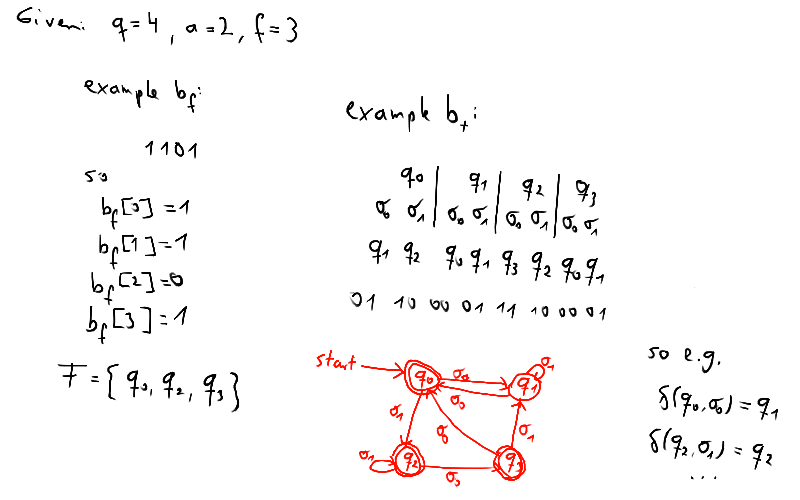
\includegraphics[width=\linewidth]{images/dfa_enum_bit_fields.png}
	\caption{Example for two possible configurations of the bit-fields $b_f$ and $b_t$ given $q, a$ and $f$. Below the corresponding DFA is drawn.}
	\label{fig:dfa_enum_bit_fields}
\end{figure}

% how to compute next DFA

Given an enumeration state $b_f, b_t$ and $q, a, f$ we will then compute the next DFA based on this state as follows. We will treat both bit-fields as numbers, $b_f$ as binary and $b_t$ as $\log_2(q)$-ary. To get to the next DFA, we will first increment $b_t$ by $1$. If $b_t = 1 \ldots 1$, then we increment $b_f$ until it contains $f$ ones (again) and set $b_t$ to $0 \ldots 0$. This behaviour is summarized in the following algorithm: \gregor{Clarify what happens at 11111...}
\vspace{0.2cm}
\begin{algorithmic}[1]
	\Function{IncrementEnumProgress\ }{$b_f, b_t, q, a, f$}
	\State add $1$ to $(b_t)_2$
	\If {$b_t = 0 \ldots 0$}
		\While {$\#_1(b_f) \neq f$}
			\State add $1$ to $(b_f)_2$
			\If {$b_f = 0\ldots 0$}
				\State \Return $\bot$
			\EndIf
		\State $b_t = 0 \ldots 0$
		\EndWhile
	\EndIf
	\State \Return $b_f, b_t$
	\EndFunction
\end{algorithmic}
\vspace{0.2cm}
The example in figure~\ref{fig:dfa_enum_incr} illustrates such increments.

% EX -- example of an enumProgress increment

\begin{figure}
	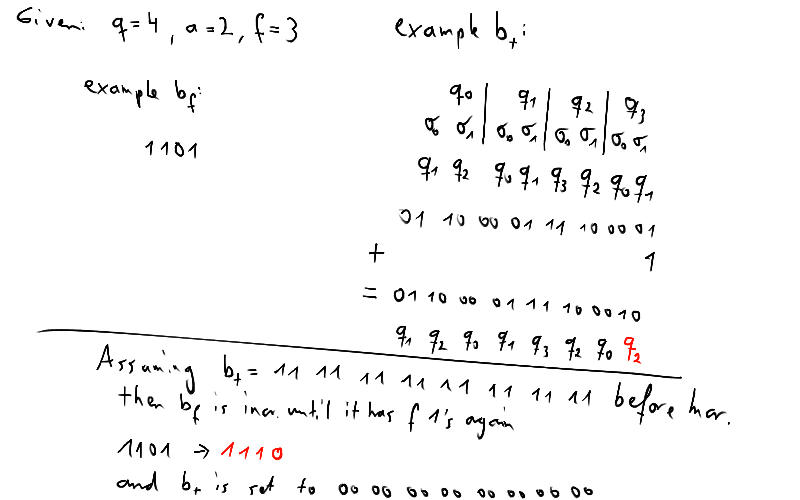
\includegraphics[width=\linewidth]{images/dfa_enum_incr.png}
	\caption{The upper half shows how a $b_t$-increment results in a change in the resulting DFAs transition function: $\delta(q_3, \sigma_1) = q_1$ becomes $\delta(q_3, \sigma_1) = q_2$. The lower half shows what happens, if $b_t$ has reached its end.}
	\label{fig:dfa_enum_incr}
\end{figure}

Based on the incremented bit-fields the new DFA can be build according to the semantics defined above:
\vspace{0.2cm}
\begin{algorithmic}[1]
	\Function{DFAfromEnumProgress\ }{$b_f, b_t, f$}
	\State $Q \gets \{q_0, \ldots, q_{q-1}\}$
	\State $\Sigma \gets \{\sigma_0, \ldots, \sigma_{a-1}\}$
	\State $\delta \gets \emptyset$
	\For {$i$ \textbf{in} $[0, \ldots, q-1]$}
		\For {$j$ \textbf{in} $[0, \ldots, a-1]$}
			\State $\delta \gets \delta \cup \{((q_i, \sigma_j), q_{b_t[i * a + j]})\}$
		\EndFor
	\EndFor
	\State $s \gets q_0$
	\State $F \gets \{ q_i | i \in [0, \ldots, q-1] \land b_f[i] = 1 \}$
	\State \Return $(Q, \Sigma, \delta, s, F)$
	\EndFunction
\end{algorithmic}
\vspace{0.2cm}
The initial bit-field values are each time $0\ldots 0$. Note how construction and use of these bit-fields results in DFAs with correct alphabet size and number of (final) states. We define $Q$ and $\Sigma$ as in the random generation method. An enumeration can finish either because a matching DFA has been found or all DFAs have been enumerated \gregor{More, beautiful, explanation. Find proper place.}

% saving enumProgress for later progression

Once the enumeration within a call of \textsc{BuildNewMinimalDFA} has been finished, it is reasonable to save the progress (meaning the current content of $b_f, b_t$), such that during the next call enumeration can be resumed from that point on. The alternative would mean, that the enumeration is run in its entirety until that point, whereas all so far found DFAs would be found used. Thus we introduce a second database $DB2$ with the following table:
\begin{center}
	\begin{tabular}{c c c c c c}
		$|Q_A|$ & |$\Sigma_A$| & $b_f$ & $b_t$
	\end{tabular}
\end{center}
We reduce the enumeration room for each calculation.
\vspace{0.2cm}
\begin{algorithmic}[1]
	\Function{BuildNewMinimalDFA-3b\ }{$q, a, f, m_{min}, m_{max}, p$}
	
		\vspace{0.2cm}
	
		\State $l \gets$ all DFAs in DB1 matching $q, a, f, m_{min}, m_{max}, p$
		\State $b_f, b_t \gets$ load enumeration progress for $q, a, f, p$ from DB2
		
		\vspace{0.2cm}
		
		\While {True}
		
			\vspace{0.2cm}
		
			\If {$b_f, b_t$ is finished}
				\State save $b_f, b_t$
				\State\Return $\bot$
			\EndIf
			\State $A_{test} \gets$ next DFA based on $b_f, b_t$
			
			\vspace{0.2cm}
			
			\If {$A_{test}$ not minimal \textbf{or not} $m_{min} \leq \mmD(A_{test}) \leq m_{max}$}
				\State \textbf{continue}
			\EndIf
			
			\If {$p = 1$ \textbf{and} $A_{test}$ is not planar}
				\State \textbf{continue}
			\EndIf
			
			\If {$A_{test}$ is isomorph to any DFA in $l$}
				\State \textbf{continue}
			\EndIf
			
			\vspace{0.2cm}
			
			\State save $b_f, b_t$ in DB2
			\State save $A_{test}$ and its respective properties in DB1
			\State\Return $A_{test}$
		\EndWhile
	\EndFunction
\end{algorithmic}
\vspace{0.2cm}

\subsection{Ideas for more efficiency}

incrementing final state binary faster in enum-alternative

speed up isomorphy test

rewrite everything in C

solve P vs NP

\section{Building directly minimal DFAs}

\subsection{Research}

\subsection{Building $m(i)$ bottom up}

Build $m$ from $m$-\MinMark\ iteratively. (Why would this basically result in running \MinMark\ all the time?)
